% Created by tikzDevice version 0.10.1 on 2016-08-25 15:40:47
% !TEX encoding = UTF-8 Unicode
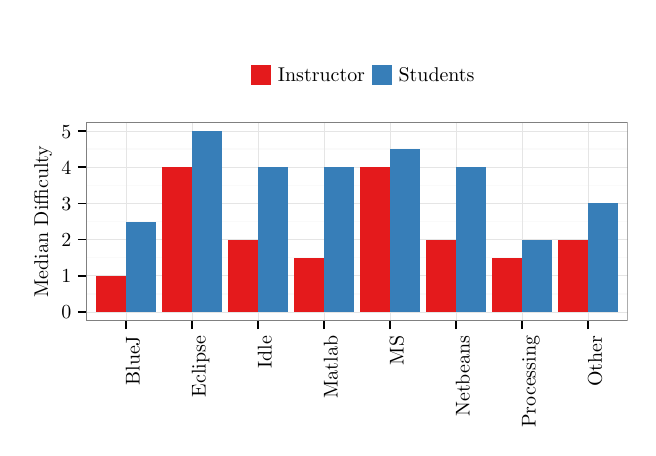
\begin{tikzpicture}[x=1pt,y=1pt]
\definecolor{fillColor}{RGB}{255,255,255}
\path[use as bounding box,fill=fillColor,fill opacity=0.00] (0,0) rectangle (216.81,144.54);
\begin{scope}
\path[clip] (  0.00,  0.00) rectangle (216.81,144.54);
\definecolor{drawColor}{RGB}{255,255,255}
\definecolor{fillColor}{RGB}{255,255,255}

\path[draw=drawColor,line width= 0.6pt,line join=round,line cap=round,fill=fillColor] ( -0.00,  0.00) rectangle (216.81,144.54);
\end{scope}
\begin{scope}
\path[clip] ( 21.16, 38.59) rectangle (216.81,110.40);
\definecolor{fillColor}{RGB}{255,255,255}

\path[fill=fillColor] ( 21.16, 38.59) rectangle (216.81,110.40);
\definecolor{drawColor}{gray}{0.98}

\path[draw=drawColor,line width= 0.6pt,line join=round] ( 21.16, 48.38) --
	(216.81, 48.38);

\path[draw=drawColor,line width= 0.6pt,line join=round] ( 21.16, 61.44) --
	(216.81, 61.44);

\path[draw=drawColor,line width= 0.6pt,line join=round] ( 21.16, 74.49) --
	(216.81, 74.49);

\path[draw=drawColor,line width= 0.6pt,line join=round] ( 21.16, 87.55) --
	(216.81, 87.55);

\path[draw=drawColor,line width= 0.6pt,line join=round] ( 21.16,100.61) --
	(216.81,100.61);
\definecolor{drawColor}{gray}{0.90}

\path[draw=drawColor,line width= 0.2pt,line join=round] ( 21.16, 41.86) --
	(216.81, 41.86);

\path[draw=drawColor,line width= 0.2pt,line join=round] ( 21.16, 54.91) --
	(216.81, 54.91);

\path[draw=drawColor,line width= 0.2pt,line join=round] ( 21.16, 67.97) --
	(216.81, 67.97);

\path[draw=drawColor,line width= 0.2pt,line join=round] ( 21.16, 81.02) --
	(216.81, 81.02);

\path[draw=drawColor,line width= 0.2pt,line join=round] ( 21.16, 94.08) --
	(216.81, 94.08);

\path[draw=drawColor,line width= 0.2pt,line join=round] ( 21.16,107.13) --
	(216.81,107.13);

\path[draw=drawColor,line width= 0.2pt,line join=round] ( 35.47, 38.59) --
	( 35.47,110.40);

\path[draw=drawColor,line width= 0.2pt,line join=round] ( 59.33, 38.59) --
	( 59.33,110.40);

\path[draw=drawColor,line width= 0.2pt,line join=round] ( 83.19, 38.59) --
	( 83.19,110.40);

\path[draw=drawColor,line width= 0.2pt,line join=round] (107.05, 38.59) --
	(107.05,110.40);

\path[draw=drawColor,line width= 0.2pt,line join=round] (130.91, 38.59) --
	(130.91,110.40);

\path[draw=drawColor,line width= 0.2pt,line join=round] (154.77, 38.59) --
	(154.77,110.40);

\path[draw=drawColor,line width= 0.2pt,line join=round] (178.63, 38.59) --
	(178.63,110.40);

\path[draw=drawColor,line width= 0.2pt,line join=round] (202.49, 38.59) --
	(202.49,110.40);
\definecolor{fillColor}{RGB}{55,126,184}

\path[fill=fillColor] ( 35.47, 41.86) rectangle ( 46.21, 74.49);
\definecolor{fillColor}{RGB}{228,26,28}

\path[fill=fillColor] ( 24.74, 41.86) rectangle ( 35.47, 54.91);
\definecolor{fillColor}{RGB}{55,126,184}

\path[fill=fillColor] ( 59.33, 41.86) rectangle ( 70.07,107.13);
\definecolor{fillColor}{RGB}{228,26,28}

\path[fill=fillColor] ( 48.60, 41.86) rectangle ( 59.33, 94.08);
\definecolor{fillColor}{RGB}{55,126,184}

\path[fill=fillColor] ( 83.19, 41.86) rectangle ( 93.93, 94.08);
\definecolor{fillColor}{RGB}{228,26,28}

\path[fill=fillColor] ( 72.46, 41.86) rectangle ( 83.19, 67.97);
\definecolor{fillColor}{RGB}{55,126,184}

\path[fill=fillColor] (107.05, 41.86) rectangle (117.79, 94.08);
\definecolor{fillColor}{RGB}{228,26,28}

\path[fill=fillColor] ( 96.32, 41.86) rectangle (107.05, 61.44);
\definecolor{fillColor}{RGB}{55,126,184}

\path[fill=fillColor] (130.91, 41.86) rectangle (141.65,100.61);
\definecolor{fillColor}{RGB}{228,26,28}

\path[fill=fillColor] (120.18, 41.86) rectangle (130.91, 94.08);
\definecolor{fillColor}{RGB}{55,126,184}

\path[fill=fillColor] (154.77, 41.86) rectangle (165.51, 94.08);
\definecolor{fillColor}{RGB}{228,26,28}

\path[fill=fillColor] (144.04, 41.86) rectangle (154.77, 67.97);
\definecolor{fillColor}{RGB}{55,126,184}

\path[fill=fillColor] (178.63, 41.86) rectangle (189.37, 67.97);
\definecolor{fillColor}{RGB}{228,26,28}

\path[fill=fillColor] (167.90, 41.86) rectangle (178.63, 61.44);
\definecolor{fillColor}{RGB}{55,126,184}

\path[fill=fillColor] (202.49, 41.86) rectangle (213.23, 81.02);
\definecolor{fillColor}{RGB}{228,26,28}

\path[fill=fillColor] (191.76, 41.86) rectangle (202.49, 67.97);
\definecolor{drawColor}{gray}{0.50}

\path[draw=drawColor,line width= 0.6pt,line join=round,line cap=round] ( 21.16, 38.59) rectangle (216.81,110.40);
\end{scope}
\begin{scope}
\path[clip] (  0.00,  0.00) rectangle (216.81,144.54);
\definecolor{drawColor}{RGB}{0,0,0}

\node[text=drawColor,anchor=base east,inner sep=0pt, outer sep=0pt, scale=  0.72] at ( 15.76, 39.38) {0};

\node[text=drawColor,anchor=base east,inner sep=0pt, outer sep=0pt, scale=  0.72] at ( 15.76, 52.43) {1};

\node[text=drawColor,anchor=base east,inner sep=0pt, outer sep=0pt, scale=  0.72] at ( 15.76, 65.49) {2};

\node[text=drawColor,anchor=base east,inner sep=0pt, outer sep=0pt, scale=  0.72] at ( 15.76, 78.54) {3};

\node[text=drawColor,anchor=base east,inner sep=0pt, outer sep=0pt, scale=  0.72] at ( 15.76, 91.60) {4};

\node[text=drawColor,anchor=base east,inner sep=0pt, outer sep=0pt, scale=  0.72] at ( 15.76,104.65) {5};
\end{scope}
\begin{scope}
\path[clip] (  0.00,  0.00) rectangle (216.81,144.54);
\definecolor{drawColor}{RGB}{0,0,0}

\path[draw=drawColor,line width= 0.6pt,line join=round] ( 18.16, 41.86) --
	( 21.16, 41.86);

\path[draw=drawColor,line width= 0.6pt,line join=round] ( 18.16, 54.91) --
	( 21.16, 54.91);

\path[draw=drawColor,line width= 0.6pt,line join=round] ( 18.16, 67.97) --
	( 21.16, 67.97);

\path[draw=drawColor,line width= 0.6pt,line join=round] ( 18.16, 81.02) --
	( 21.16, 81.02);

\path[draw=drawColor,line width= 0.6pt,line join=round] ( 18.16, 94.08) --
	( 21.16, 94.08);

\path[draw=drawColor,line width= 0.6pt,line join=round] ( 18.16,107.13) --
	( 21.16,107.13);
\end{scope}
\begin{scope}
\path[clip] (  0.00,  0.00) rectangle (216.81,144.54);
\definecolor{drawColor}{RGB}{0,0,0}

\path[draw=drawColor,line width= 0.6pt,line join=round] ( 35.47, 35.59) --
	( 35.47, 38.59);

\path[draw=drawColor,line width= 0.6pt,line join=round] ( 59.33, 35.59) --
	( 59.33, 38.59);

\path[draw=drawColor,line width= 0.6pt,line join=round] ( 83.19, 35.59) --
	( 83.19, 38.59);

\path[draw=drawColor,line width= 0.6pt,line join=round] (107.05, 35.59) --
	(107.05, 38.59);

\path[draw=drawColor,line width= 0.6pt,line join=round] (130.91, 35.59) --
	(130.91, 38.59);

\path[draw=drawColor,line width= 0.6pt,line join=round] (154.77, 35.59) --
	(154.77, 38.59);

\path[draw=drawColor,line width= 0.6pt,line join=round] (178.63, 35.59) --
	(178.63, 38.59);

\path[draw=drawColor,line width= 0.6pt,line join=round] (202.49, 35.59) --
	(202.49, 38.59);
\end{scope}
\begin{scope}
\path[clip] (  0.00,  0.00) rectangle (216.81,144.54);
\definecolor{drawColor}{RGB}{0,0,0}

\node[text=drawColor,rotate= 90.00,anchor=base east,inner sep=0pt, outer sep=0pt, scale=  0.72] at ( 40.43, 33.19) {BlueJ};

\node[text=drawColor,rotate= 90.00,anchor=base east,inner sep=0pt, outer sep=0pt, scale=  0.72] at ( 64.29, 33.19) {Eclipse};

\node[text=drawColor,rotate= 90.00,anchor=base east,inner sep=0pt, outer sep=0pt, scale=  0.72] at ( 88.15, 33.19) {Idle};

\node[text=drawColor,rotate= 90.00,anchor=base east,inner sep=0pt, outer sep=0pt, scale=  0.72] at (112.01, 33.19) {Matlab};

\node[text=drawColor,rotate= 90.00,anchor=base east,inner sep=0pt, outer sep=0pt, scale=  0.72] at (135.87, 33.19) {MS};

\node[text=drawColor,rotate= 90.00,anchor=base east,inner sep=0pt, outer sep=0pt, scale=  0.72] at (159.73, 33.19) {Netbeans};

\node[text=drawColor,rotate= 90.00,anchor=base east,inner sep=0pt, outer sep=0pt, scale=  0.72] at (183.59, 33.19) {Processing};

\node[text=drawColor,rotate= 90.00,anchor=base east,inner sep=0pt, outer sep=0pt, scale=  0.72] at (207.45, 33.19) {Other};
\end{scope}
\begin{scope}
\path[clip] (  0.00,  0.00) rectangle (216.81,144.54);
\definecolor{drawColor}{RGB}{0,0,0}

\node[text=drawColor,rotate= 90.00,anchor=base,inner sep=0pt, outer sep=0pt, scale=  0.72] at (  7.36, 74.49) {Median Difficulty};
\end{scope}
\begin{scope}
\path[clip] (  0.00,  0.00) rectangle (216.81,144.54);
\definecolor{fillColor}{RGB}{255,255,255}

\path[fill=fillColor] ( 72.21,118.93) rectangle (165.76,136.00);
\end{scope}
\begin{scope}
\path[clip] (  0.00,  0.00) rectangle (216.81,144.54);
\definecolor{fillColor}{RGB}{228,26,28}

\path[fill=fillColor] ( 80.80,123.91) rectangle ( 87.92,131.02);
\end{scope}
\begin{scope}
\path[clip] (  0.00,  0.00) rectangle (216.81,144.54);
\definecolor{fillColor}{RGB}{55,126,184}

\path[fill=fillColor] (124.42,123.91) rectangle (131.54,131.02);
\end{scope}
\begin{scope}
\path[clip] (  0.00,  0.00) rectangle (216.81,144.54);
\definecolor{drawColor}{RGB}{0,0,0}

\node[text=drawColor,anchor=base west,inner sep=0pt, outer sep=0pt, scale=  0.72] at ( 90.43,124.99) {Instructor};
\end{scope}
\begin{scope}
\path[clip] (  0.00,  0.00) rectangle (216.81,144.54);
\definecolor{drawColor}{RGB}{0,0,0}

\node[text=drawColor,anchor=base west,inner sep=0pt, outer sep=0pt, scale=  0.72] at (134.06,124.99) {Students};
\end{scope}
\end{tikzpicture}
